% all-in-one cheatsheet layout (Michael Franzen, 2013)
\documentclass[a4paper]{article}

% geometry settings
\usepackage[top=2cm, bottom=2.5cm, left=2cm, right=2cm]{geometry}

% font settings
%\usepackage[light,math]{kurier}
\usepackage[T1]{fontenc}
\usepackage[utf8]{inputenc}
\usepackage{marvosym}
\usepackage{amssymb}
\usepackage{amsfonts}
\usepackage{amsmath}
\usepackage{amsthm}

% colors
\usepackage{xcolor}
\definecolor{lightgray}{gray}{0.8}

% formatting
\usepackage{paralist}
\usepackage{multicol}
\usepackage{tabularx}
\usepackage{Tabbing}
\usepackage{booktabs}
\usepackage{fancyhdr}
\usepackage{url}
\usepackage[framemethod=tikz]{mdframed}
\pagestyle{fancy}

% math
\usepackage{array}
\usepackage{eqnarray}
\usepackage{mathtools}

% figures
\usepackage{wrapfig}
\usepackage{subfig}

% figure modules
\usepackage{graphicx}
\usepackage{tikz}
\usetikzlibrary{positioning,calc, shapes}
\usepackage{algorithm2e}
\usepackage{verbatim}	

% TOC & Glossary
\usepackage{sectsty}
\usepackage[nottoc,notlof,notlot]{tocbibind}
\usepackage[titles,subfigure]{tocloft}

% commands
\usepackage{xargs}
\usepackage{ifthen}

% head line
\fancyhf{}
\chead{Graph Theory - Sheet 3 - \today\\J. Batzill (1698622), M. Franzen (1696933), J. Labeit (1656460)}
\renewcommand{\headrulewidth}{0.4pt} %obere Trennlinie

\newcommand{\sheetnumber}{1}

% (problem number)
\surroundwithmdframed[
    hidealllines=true,
    backgroundcolor=gray!10,
    skipbelow=\baselineskip,
    skipabove=\baselineskip
]{mylemma}

\surroundwithmdframed[
	linecolor=white,
	skipbelow=\baselineskip,
	skipabove=\baselineskip
]{mytheorem}




\begin{document}
	
	\newtheorem{mytheorem}{Theorem}[section]
	\newtheorem{mylemma}{Lemma}[mytheorem]	

	\newenvironmentx*{solution}[1]{\section*{Problem #1}\addtocounter{section}{1}\setcounter{mylemma}{0}\setcounter{mytheorem}{0}}{}
	\newenvironmentx*{theorem}[1]{\begin{mytheorem}#1\\\begin{proof}}{\end{proof}\end{mytheorem}}
	\newenvironmentx*{lemma}[1]{\begin{mylemma}#1\\\begin{proof}}{\end{proof}\end{mylemma}}


	\begin{solution}{9}
		\begin{theorem}{A hypercube $Q_n$ is Hamiltonian. It has a girth of $4$ for $n \geq 2$ and $\infty$ otherwise. It's diameter is $n$, it's order $2^n$ and it has a size of ?.}
			Let $S$ be a set of cardinality $|S| = n$. We construct $Q_n = (V_Q, E_Q)$ by creating a vertex for each subset of $S$ and moreover add edges between those subsets which differ by only one element. In the following, we will use binary representations of the vertices of $Q_n$ since $V_Q = \mathcal{P}(S) \cong (\mathbb{Z}/2\mathbb{Z})^n$ (we can denote a $1$ for including an element and a $0$ for excluding an element in a subset).\\

			\textbf{Order:} Since $V_Q = \mathcal{P}(S)$ and $|\mathcal{P}(S)| = 2^n$, \emph{the order of $Q_n$ is $2^n$.}\\

			\textbf{Size:}\\

			\textbf{Girth:} We differ between two cases.
				\begin{itemize}
					\item \textbf{Case 1: } $n=1$. Our graph contains exactly one edge and is therefore acyclic. \emph{Hence, the girth is $\infty$ for $n=1$.}

					\item \textbf{Case 2: } $n\geq2$ Our graph contains the cycle ($\emptyset$, $\{a\}$, $\{a,b\}$, $\{b\}$, $\emptyset$) $(a,b \in S)$ which has length $4$.

						A shorter cycle ($A$, $B$, $C$, $A$) $(A, B, C \in V_Q)$ does not exist due to the property that two adjacent vertices differ by exactly one element. For such a cycle, $B$ and $A$ differed by one element, and hence $A$ and $C$ differed by two or are equal. However, a difference of zero or two elements between two consecutive elements renders any walk invalid. The edge $\{C, A\}$ could not be contained in $Q_n$.
 
						\emph{From these considerations, for $n \geq 2$, the girth is $4$.}
				\end{itemize}

			\textbf{Diameter:}
				For any set $A \in V_Q$, we are able to get to any other element $B \in V_Q$ by inserting or removing a maximum of $n$ elements. Thus, a path of length $n$ is sufficient to walk from any $A$ to any $B$. Furthermore, there exist $A$ and $B$ such that a path of length $n$ is the shortest path between them. E.g. $A = \emptyset \in V_Q$, $B = S \in V_Q$. \emph{Thus, the diameter of $Q_n$ is $n$.}\\

			\textbf{Hamiltonian:} A Hamiltonian cycle is equivalent to an enumeration of $(\mathbb{Z}/2\mathbb{Z})^n$ in which consecutive elements differ by exactly one element. We provide such an enumeration: the \emph{Gray Code\footnote{For $n=2$: $00$,$01$,$11$,$10$,$00$. Generally, the $k$'th vertex in the Hamiltonian cycle is $k \otimes \lfloor \frac{k}{2} \rfloor$ whereby $\cdot \otimes \cdot$ denotes the exclusive or.}}. \emph{Thus, there exists a Hamiltonian cycle and $Q_n$ is Hamiltonian.}
		\end{theorem}

		\newpage		

		\begin{theorem}{A complete bipartite graph $K_{m, n}$ is Hamiltonian iff $m = n$. It's girth is $4$ for $m, n \neq 1$ and and $\infty$ otherwise. It's diameter is $1$ for $m = n = 1$ and $2$ otherwise. The graph's order is $m + n$ and it's size is $m \cdot n$.}
			Let $V = \{v_1, ..., v_m\}$ and $W = \{w_1, ..., w_n\}$ denote the two partitions of $K_{m, n} = (V_K, E_K)$.\\

			\textbf{Order:} The first partition has $m$ elements, the second $n$ elements. \emph{Thus, $K_{m,n}$ has an order of $m + n$.}\\

			\textbf{Size:} Each of the $m$ elements of the first partition are connected to each of the $n$ elements in the second partition. \emph{Thus, $K_{m,n}$ has a size of $m \cdot n$}.\\

			\textbf{Girth:} If either $m=1$ or $n=1$, then all vertices of one partition are indicent to and only to the single vertex of the other partition. Hence, there is no cycle in $K_{1, n}$ or $K_{m, 1}$ and \emph{the girth of $K_{m,n}$ is $\infty$ if $n = 1$ or $m=1$}.\\

				If $m, n \neq 1$, each cycle must have even length since any two consectuive vertices in a path of $K_{n,m}$ are in different partitions. Thus, we require an even amount of edge-crossings to enclose a walk. Any cycle has a length of at least $3$, thus the girth of $K_{m,n}$ has to exceed or be equal to $4$.

				Furthermore, we find such a cycle of length $4$ easily since both partitions $V, W$ have at least $2$ vertices: $(v_1, w_1, v_2, w_2, v_1)$. \emph{From these considerations, the girth of $K_{m,n}$ must be equal to $4$.}\\

			\textbf{Diameter:} For $m = n = 1$, there are exactly two vertices in different partitions. They have a distance of $1$ and thus, \emph{the diameter of $K_{1,1}$ is $1$}.\\

				Since two consectuive vertices in a path of $K_{n,m}$ are in different partitions $V, W$ the distance between two vertices in the same partition has to be at least $2$. Moreover, we find a path of distance $2$ between $v_1 \in V$ to $v_2 \in V$: $(v_1, w, v_2)$ for any $w \in W$. Thus, the diameter does not deceed $2$.

				For any two vertices in different partitions $V, W$, they are directly connected by a path of length $1$.

				 \emph{Hence, the diameter of $K_{m,n}$ is $2$ if not $m = n = 1$}.\\

			\textbf{Hamiltonian:}
		\end{theorem}
			
		\newpage

		\begin{theorem}{The Petersen graph is not Hamiltonian, it has a girth of $5$, a diameter of $2$, an order of $10$ and a size of $15$.}
			\textbf{Order:} The graph has $10$ vertices and thus, it's order is $10$.\\
			
			\textbf{Size:} The graph has $15$ edges and thus, it's size is $15$.\\

			\textbf{Girth:} \\

			\textbf{Diameter:} \\

			\textbf{Hamiltonian:}

		\end{theorem}
	\end{solution}
	\newpage
	\begin{solution}{11}
		For each even integer $k > 1$, the complete graph $K_{(n+1)}$ is a $k$-regular graph with no 1-factor. 
		For each odd $k > 1$ we can construct a k-regular graph with no 1-factor in the following way. \\
		In order to garantee that the graph has no 1-factor we can use Tutt's theorem. 
		We construct the graph by starting of with one vertex $v$ connected to k subgraphs $S$ which are not inter-connected. 
		\begin{figure}[h]
			\centering
			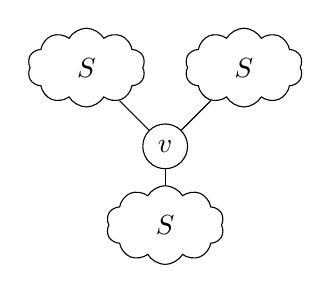
\begin{tikzpicture}
				\node[cloud, cloud puffs=10, cloud puff arc=120, aspect=2, minimum width=1.5cm, minimum height=1cm, draw] (S1)  at (0,-1.0) {$S$};
				\node[cloud, cloud puffs=10, cloud puff arc=120, aspect=2, minimum width=1.5cm, minimum height=1cm, draw] (S2)  at (-1.0,1.0) {$S$};
				\node[cloud, cloud puffs=10, cloud puff arc=120, aspect=2, minimum width=1.5cm, minimum height=1cm, draw] (S3)  at (1.0,1.0) {$S$};

				\node[circle, draw] (v) at (0, 0) {$v$};
				\draw(v) -- (S1);
				\draw(v) -- (S2);
				\draw(v) -- (S3);
			\end{tikzpicture}
		\caption{Example with k=3}
		\end{figure}
		Then we construct $S=(V,E)$ in such a way that $|V|$ is odd and that all vertices in $V$ have degree k except of one vertex $u \in V$ with degree $k-1$. 
		If we then connect $u$ to $v$ we get a k-regular graph. 
		Using Tutt's theorem we know that the resulting graph has no 1-factor. 
		Because if $v$ is removed we get $k$ components $S$ with odd number of vertices and $k$ is greater than 1.\\ \\
		
		In order to contruct $S$ we first need the following lemma.
		\begin{lemma}{For any odd integer $k > 1$ it is possible to construct $(k-1)$-regular graph $G=(V,E)$ with $k+1$ vertices.}
			We can obtain $G$ from $K_{k+1}$ by removing by removing all the edges from $K_{k+1}$ contained in a perfect matching. 
			By removing the edges the degree of every vertex decreases exactly by one. 
			$K_{k+1}$ is by definition $k$-regular, hence $G$ is $k-1$-regular. 
			A perfect matching in $K_{k+1}$ exists, because $k+1$ is even, and the condition from Tutte's theorem always holds in a complete graph. 
			To find such a matching we can just randomly choose $(u,v)$ edges and remove $u$ and $v$ from $K_{k+1}$. 
		\end{lemma}
		
		
		\emph{Constructing a connected graph $S=(V,E)$ with $|V|=k+2$ and the degree sequence $( k,k,...,k,(k-1))$. }  
		First we construct a $(k-1)$-regular graph $S' = (V',E')$ with $k+1$ vertices as described in the lemma. 
		Then we can add one vertex to $S'$ and connect it to all vertices in $V'$ except of one vertex. 
		Thus we get a new graph $S$. 
		Because we only added one vertex $|V| = |V'| +1 = k+2$ and the degree of the newly added vertex is $k$.
		The degree of all the other vertices except of the last one is increased by one. 
		Hence, $S$ hat the degree sequence $(k,k,...,k,(k-1))$. 
		\begin{figure}[h]
			\centering
			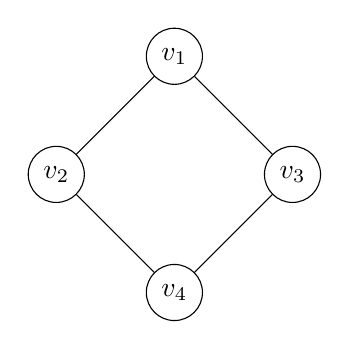
\begin{tikzpicture}
				\node[circle, draw] (v1) at (0, 1.5) {$v_1$};
				\node[circle, draw] (v2) at (-1.5, 0) {$v_2$};
				\node[circle, draw] (v3) at (1.5, 0) {$v_3$};
				\node[circle, draw] (v4) at (0, -1.5) {$v_4$};
				
				\draw(v1) -- (v2);
				\draw(v1) -- (v3);
				\draw(v3) -- (v4);
				\draw(v2) -- (v4);
			\end{tikzpicture}
			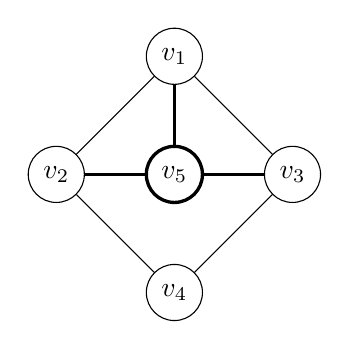
\begin{tikzpicture}
				\node[circle, draw] (v1) at (0, 1.5) {$v_1$};
				\node[circle, draw] (v2) at (-1.5, 0) {$v_2$};
				\node[circle, draw] (v3) at (1.5, 0) {$v_3$};
				\node[circle, draw] (v4) at (0, -1.5) {$v_4$};
				\node[circle, draw,very thick] (v5) at (0, 0) {$v_5$};
				
				\draw(v1) -- (v2);
				\draw(v1) -- (v3);
				\draw(v3) -- (v4);
				\draw(v2) -- (v4);
				\draw[very thick](v5) -- (v1);
				\draw[very thick](v5) -- (v2);
				\draw[very thick](v5) -- (v3);
			\end{tikzpicture}
		\caption{$S'$ and $S$ for k=3}
		\end{figure}
	\end{solution}
	\newpage
	\begin{solution}{12}
	In the following I will show that any graph $G$ with $2n$ vertices and all degrees at least $n$ has a 1-factor. 	
	I will show that if we divide such a $G$ into two parts we can remove edges until we get an bipartite 1-regular graph. 
	Then using the corollary of Hall's theorem we know we can find a perfect matching.
		\begin{theorem}{Let $G=(V,E)$ be a graph with $|V| = 2n$ vertices with all degree atleast n, then $G$ has a 1-factor.}
		Because $|V| = 2n$ we can divide the vertices $V$ into two subsets $A,B \subset V$ with $|A|=|B|=n$ and $A \cap B = \emptyset$. 
		
	
		\end{theorem}
	\end{solution}
	
\end{document}
